\documentclass[journal]{IEEEtran}
\usepackage[usenames]{color}
\usepackage{epsfig}
\usepackage{graphics}
\usepackage{caption}
\usepackage{amsmath}
\usepackage{amssymb}
\usepackage{multirow}
\usepackage{cite}
\usepackage{array}
\usepackage{pslatex} 
\usepackage{url}
\usepackage{lineno}
\usepackage{graphicx}  % Written by David Carlisle and Sebastian Rahtz
\usepackage{setspace}
\usepackage{tikz}
\usepackage{hhline}
\usepackage{mathtools}
\usepackage{caption}
\usepackage{xcolor}
\usepackage{algorithm}
\usepackage{algorithmic}
\usepackage{placeins}

\usepackage[letterpaper]{geometry}
\geometry{verbose,tmargin=0.7in,bmargin=0.7in,lmargin=0.65in,rmargin=0.65in}
\setlength{\headheight}{17pt}
%\captionsetup{labelfont={up},font=small}
\captionsetup[figure]{name={Fig.},labelsep=period,font=small}
\captionsetup[table]{name={TABLE},labelsep=period,font=small}

\usepackage{abstract}
\renewcommand{\absnamepos}{flushleft}
\setlength{\absleftindent}{0pt}
\setlength{\absrightindent}{0pt}


% If IEEEtran.cls has not been installed into the LaTeX system files,
% manually specify the path to it like:
% \documentclass[journal]{../sty/IEEEtran}


\usepackage{amsmath}   % From the American Mathematical Society
\hyphenation{}

% This is to insert comments
\newcommand{\memoA}[1]{{\textcolor{red}{\bf{$<$\emph{#1}$>$}}}}
\newcommand{\memoB}[1]{{\textcolor{magenta}{\bf{$<$\emph{#1}$>$}}}}
\newcommand{\memoC}[1]{{\textcolor{blue}{\bf{$<$\emph{#1}$>$}}}}
\newcommand{\memoD}[1]{{\textcolor{green}{\bf{$<$\emph{#1}$>$}}}}

% This is to automatically remove them
%\renewcommand{\memoA}[1]{}
%\renewcommand{\memoB}[1]{}
%\renewcommand{\memoC}[1]{}
%\renewcommand{\memoD}[1]{}
%\renewcommand{\efloatseparator}{\mbox{}}
%\renewcommand{\theposttbl}{\Roman{posttbl}}


%%%% Subfigures %%%%%%%%%%%%%%%%%%%%%%%%%%%%%%%

%\renewcommand\setlength{1cm}

%%%%% MC 16/05/06 THIS IS FOR VHDL LANGUAGE %%%%% 
\usepackage{listings}
\lstset{language=[AMS]VHDL}
\lstset{basicstyle=\verbatim@font} 

%%%%%%%%%%%%%%%%%%%%%%%%%%%%%%%%%%%%%%%%%%%%%%%%%%
% The paper headers
% correct bad hyphenation here
\pagenumbering{gobble} 

% The paper headers
\usepackage[english]{babel}
\usepackage[utf8]{inputenc}
\usepackage{fancyhdr}
\pagestyle{fancy}
\fancyhf{}
\lhead{\textcolor{violet}{\Large\textbf{IEEE EMB}}}
\rhead{\textcolor{violet}{\Large\textbf{\textsc{Med          }}} \thepage}
%\fancyfoot[CE,CO]{\leftmark}
\pagestyle{fancyplain}


\title{\textcolor{violet}{Predicting Severity of COVID-19 From Patients' Chest CT Images Using Self-Supervised Image Segmentation Approaches}}


\begin{document}

% \begin{flushright} 
% AAAAAAAAAAAAAAAAAAAAAAAAAAAAAAAAAAAAa
% \end{flushright}.	
% \begingroup
%\let\newpage\relax% Void the actions of \newpage
%	\maketitle\thispagestyle{fancy}   
%\endgroup

%
%
% author names and IEEE memberships
% note positions of commas and nonbreaking spaces ( ~ ) LaTeX will not break
% a structure at a ~ so this keeps an author's name from being broken across
% two lines.
% use \thanks{} to gain access to the first footnote area
% a separate \thanks must be used for each paragraph as LaTeX2e's \thanks
% was not built to handle multiple paragraphs
%\author{Michael~Shell,~\IEEEmembership{Member,~IEEE,}
%        John~Doe,~\IEEEmembership{Fellow,~OSA,}
%        and~Jane~Doe,~\IEEEmembership{Life~Fellow,~IEEE}% <-this % stops a space

\author{\textbf{Daryl Fung, PingZhao. Hu, Carson Leung, Qian Liu, Judah Zammit}\\
\vspace*{0.1cm}

\small
University of Manitoba, MB, Canada\\

\normalsize
	
	%\thanks{Manuscript received January 20, 2002; revised November 18, 2002.
	%        This work was supported by the IEEE.}% <-this % stops a space
	%\thanks{M. Shell is with the Georgia Institute of Technology.}}
	%\thanks{This paragraph of the first footnote will contain the date on which you submitted your paper for review. It will also
}

% note the % following the last \IEEEmembership and also the first \thanks - 
% these prevent an unwanted space from occurring between the last author name
% and the end of the author line. i.e., if you had this:
% 
% \author{....lastname \thanks{...} \thanks{...} }
%                     ^------------^------------^----Do not want these spaces!
%
% a space would be appended to the last name and could cause every name on that
% line to be shifted left slightly. This is one of those "LaTeX things". For
% instance, "A\textbf{} \textbf{}B" will typeset as "A B" not "AB". If you want
% "AB" then you have to do: "A\textbf{}\textbf{}B"
% \thanks is no different in this regard, so shield the last } of each \thanks
% that ends a line with a % and do not let a space in before the next \thanks.
% Spaces after \IEEEmembership other than the last one are OK (and needed) as
% you are supposed to have spaces between the names. For what it is worth,
% this is a minor point as most people would not even notice if the said evil
% space somehow managed to creep in.
%





\twocolumn[
\begin{@twocolumnfalse}
    \maketitle\thispagestyle{fancy}   
%	\begin{abstract}
		\noindent
		\textcolor{violet}{\textbf{ABSTRACT}} COVID-19 is the new outbreak of a contagious disease that infects the lungs. Currently, no vaccines or antiviral medicines exist for COVID-19 as COVID-19 is a newly infectious disease that was first discovered around December 2019. As COVID-19 is a very contagious disease, cases appear faster than the amount of test kit available. Currently, the most common testing used is PCR(Polymerase Chain Reaction) test. These test samples are sent to a centralized lab for analysis which would take several days for the test results to be available. Due to the exponential rate of infections, the limited amount of test kits, and the long wait time for the test results to be available, many infected patients are unable to get tested and receive treatments. An alternative approach to test for COVID-19 patients is through computerized tomography (CT) scan of the lungs. CT scan can drastically reduce the time taken for test results to be available and this could speed up the testing time as well as the limiting number of testing kits available. We will propose a deep learning architecture that can evaluate different segmentation of the lungs from CT images to detect if a patient is infected with COVID-19 so that we can reduce the amount of time taken to carry out testing to determine if patients are infected with COVID-19. In addition, we will calculate the severity of the lungs affected by the disease from the CT images. The lungs will be subdivided into different regions, a calculation of the severity of each region of the lungs will be carried out through evaluation of CT severity score (CT-SS) or Dice Similarity Coefficient (DSC). \\
		\\
\noindent		
\textcolor{violet}{\textbf{INDEX TERMS}}  Deep Learning, REMOVE THIS: TODO: update abstract, add multi-seg figure, add severity score performance\\
\\
\textcolor{violet}{\textbf{IMPACT STATEMENT}} The authors should include here a significance statement of no more than 30 words. The statement should summarize the main findings of the research work reported in the manuscript.
\vspace{0.5cm}
		
%	\end{abstract}
\end{@twocolumnfalse}
]

%{\small \emph{\textbf{Index Terms}} -- \textbf{Say something}}


% Note that keywords are not normally used for peerreview papers.

% For peer review papers, you can put extra information on the cover
% page as needed:
% \begin{center} \bfseries EDICS Category: 3-BBND \end{center}
%
% For peerreview papers, inserts a page break and creates the second title.
% Will be ignored for other modes.
\IEEEpeerreviewmaketitle

\section{INTRODUCTION}

\IEEEPARstart{C}{OVID-19} is a newly identified disease that is very contagious and has been rapidly spreading across different countries around the world. The virus that was first identified in Wuhan has now infected more than 3.5 million people around the whole world and causes more than 245,000 deaths. Common symptoms from COVID-19 are fever, dry cough, but in more serious cases, patients can experience difficulty in breathing. As more people are infected, communities that have been in close contact with infected patients are getting tested for COVID-19. The test used to carry out the test for COVID-19 uses Polymerase Chain Reaction (PCR) test which could take several days for the test results to be available as the test samples are sent to a centralized lab for analysis and can be time-consuming. There is a limited number of supplies of PCR tests which is a bottleneck for testing to be efficient. Several alternative methods have been considered to test patients that are COVID-19 positive including a computerized tomography (CT) scan of the lungs. CT scans of the lungs are faster and easier to detect COVID-19 presence in patients. As the number of infected patients increases exponentially, it can be hard to provide testing scans for patients because of the limited number of doctors. It is recommended that Artificial Intelligence systems are used to analyze the CT scans of lung patients to determine the infected region of the lungs with COVID-19 and monitor the disease progression as well as to compensate for the high number of patients. Convolutional Neural Network (CNN) \cite{ref1} is an important technique to be used in image processing as CNN is able to automatically captures useful features instead of handcrafting features to be used to evaluate on the segmentation of the CT lung images. Fan et al. \cite{ref2} developed InfNet that uses CNN and fully supervised method to predict the segmentation of ground-glass opacities and consolidation. Fan et al. also incorporated semi-supervised learning to enlarge the limited number of training samples for CT lung image segmentation. However, deep learning requires a large of number of samples to be able to achieve good performance. Fan et al. uses pseudo labelling as semi-supervised learning to migitate the limited number of samples but pseudo labelling can take up to 3 times the time taken to train the network when undergoing fully supervised learning.  Therefore, we propose using self-supervised deep learning to analyze and create a pixel-level segmentation of CT scan images of patients’ lungs to determine the infected area of the CT lung images that includes ground-glass opacities and consolidation. Our self-supervised learning method integrated into InfNet is less time consuming than pseudo labelling as pseudo labelling requires training InfNet on the labeled data, evaluating InfNet on the unlabeled data, then re-trained InfNet on the total dataset. Our \textit{key contribution} in this paper is to integrate self-supervision into an existing network to improve the performance of the original network. We extend the work of InfNet as InfNet is one of the high performing model that includes CNN and several techniques to segment the ground-glass opacities and the consolidation area of the CT lung images. We show that integration self-supervised learning to InfNet improves the performance of InfNet.
\section{Related works}

There are several works that have been proposed to create image segmentation for CT scan lung images of COVID-19 positive patients. They have demonstrated effective solutions using deep neural networks to accurately predict if a patient has COVID-19 positive or negative. 

A study has been conducted that uses multiple models for different tasks where the study uses both classification and image segmentation tasks for COVID-19 detection through multi-tasks learning. The study uses Inception Residual Recurrent Neural Network (IRRCNN) for the classification of COVID-19 detection and uses Nabla-Net (NABLA-N) network for infected region segmentation for X-ray and CT images scan. \cite{ref1} Transfer learning is used to retrain the IRRCNN model with samples to differentiate between COVID-19 positive samples and negative samples in the classification phase. Mathematical Morphological approaches are implemented for selecting appropriate contours for chest region selection in the segmentation phase with NABLA-N network. Some classical imaging and adaptive threshold approaches are applied to extract the features to identify infected regions of COVID-19. They used a total number of 5,216 samples of which 3,875 samples are pneumonia and 1,341 samples are normal.

Another study \cite{ref2} introduces a feature variation block and progressive atrious spatial pyramid pooling block using COVID-segNet, a high accuracy network that is able to create segmentation of COVID-19 infection from chest CT images. The network consists of an Encoder and a Decoder with residual skip connection connecting the encoder and the decoder at their respective layer, following the architecture of UNET \cite{ref3}. Their main findings include the introduction of an FV block and a PASPP block. FV block consists of three branches - contrast enhancement branch, position sensitive branch, and identity branch. These branches can enable automatic change of parameters to display positions and boundaries of COVID-19. The PASPP block takes features extracted from the FV block to acquire semantic information with a variety of receptive fields. The dataset that they used consists of 21,658 labeled chest CT images, of which 861 CT images are confirmed COVID-19. 

The paper above however conducted the study with a good amount of data samples to train the network to achieve a high performance. They obtained their dataset from hospitals through obtaining permission. We would like to create a network that does not require much labeled dataset to be able to achieve good performance. By doing this method, we could bring this network forward to detect new lung diseases when there are not much dataset available. Besides that, the paper is only able to recognize the presence of COVID-19 in a patient, but the papers could not quantify the severity of the disease. 

While there is a limited number of public data samples available for CT COVID-19 lung images segmentation, it will not be feasible to train a network to achieve high performance. There are a different number of research that resolve this issue. One method is to use semi-supervised learning to mitigate the problem of having a low number of data samples to improve the performance of deep neural networks. Instead of having to manually annotate the data, semi-supervised learningutilizes the unlabeled data samples to aid in the training for the network.

Deng Pin Fan et al. \cite{ref14} used semi-supervised learning to enlarge the limited number of training samples for CT lung image segmentation. They developed a model called InfNet and semi-InfNet. The InfNet version of the model uses fully supervised method to predict the segmentation of the CT images for ground-glass opacities and consolidations. The model outputs 4 images of the segmentation for the CT lung images that contains either ground-glass opacities or consolidations with different image sizes. The segmentation of the different image sizes are resized to the same size as the ground truth of the segmentation to compute the loss function. They also uses a edge loss to guide the model to predict the bounding area of the segmentation. To improve InfNet, they use semi-supervised by progressively enlarging the training dataset with unlabeled data using random sampling strategy. Specifically, they generate pseudo labels for unlabeled CT lung images. The advantage of using semi-supervised learning is that we can generate pseudo labels to increase the number of data samples. However, semi-supervised learning still require the unlabeled CT images before being able to undergo its learning procedure.

Another study \cite{ref27} uses Task-Based Feature Extraction Network (TFEN) and Covid-19 Identification Network (CIN).  They propose to use task-specific feature extraction network that is tailored to CT lung images with three different classes: Healthy, pneumonia, and COVID-19 cases. They also mentioned that dataset for COVID-19 is still limited and there is not enough high quality dataset. They treat the task-specific feature extraction network as autoencoders and train the overall TFEN module to extract the relevant features from the CT images. Then, they use CIN to perform classification on the extracted features from the TFEN module. Due to the fact that by providing a person with limited CT images, they can easily detect the abnormal regions and differentiate between them very accurately by making use of prior information. This helped them develop a semi-supervised feature extraction network that allows obtaining the relevant prior information to perform the classification in order to mimic human behaviours. However, this study does not undergo segmentation of the CT lung images for better diagnosis of the CT lung images. It also does not provide the severity score of the CT lung image.

%Another study \cite{ref9} uses fine-grained segmentation networks (FGSN) to produce a dense segmentation map. Instead of using manually annotated labels, they created labels in a self-supervised manner. Features were extracted in certain layers in the network and clustered using k-means clustering. The cluster assignments are then used as supervision for the training. They showed that the learned representations can contain useful information for visual localization. The performance of the model improved by as much as 15% when trained with self-supervised learning instead of just classification.

\section{Problem Statements}
There are several limitations in the related works described. First, getting a high performance in deep neural networks requires an abundant amount of annotated samples. Performance can be drastically reduced if there are not enough data samples to compensate for the model’s complexity. Second, learning complex data distributions require a higher model complexity to be able to fit the distribution with better performance. The related works utilize semi-supervised learning to increase the number of data samples to achieve higher performance. As pixel-level segmentation on CT images is a complex task, pixel-level segmentation requires a high model complexity to fit the distribution. Unfortunately, there is a limited number of publicly available COVID-19 datasets especially in the form of pixel-level segmentation. The limited number of samples available greatly reduces the performance of modeling complex distribution for pixel-level segmentation of CT scans lung images. 

To solve the challenges, We propose a model and technique that utilizes self-supervised learning to mitigate the limited number of publicly available COVID-19 CT lung images samples to segment the infected regions of CT lung images. 

\section{Methodology}


In this section, we will show the details of the self-supervised InfNet for imaging segmentation model including the network architecture, the data preprocessing steps, and the loss function. We will show how self-supervised InfNet helps to improve generalisation and performance of the model while having a limited number of data samples. We will also show the extension of our data preprocessing steps which further improves the performance of our model.

Supervised InfNet (Lung Infection Segmentation Network) will be used as our baseline to compare without using any semi-supervised learning algorithm. This is to show that the self-supervised learning method  improves the performance of the baseline supervised learning InfNet for imaging segmentation. We will extend our work on supervised InfNet by adding self-supervised method to it.

We will not change the structure of the InfNet model and use the default parameters as included in their GitHub code. There will be two different types of the InfNet model - single InfNet and multi InfNet. 

The single InfNet will create a single-labeled segmentation of the image for the infected region. The single InfNet predicts if the region is either ground-glass opacities or consolidations. It represents ground-glass opacities or consolidations as the same label. This means that the single InfNet will only predict the infected region without classifying them more specifically.  The CT lung image is first passed into the initial convolutional layers of the single InfNet to extract the features of the CT lung image. Then, the features generated from the convolutional layer are fed into the partial decoder module, reverse attention module and the edge detection module. The edge detection module is to help the network with detection of the boundaries of the segmentation. The reverse attention and the partial decoder generates the segmentation of the infection regions of the CT lung images.

The prediction from the single InfNet represent the infected region and will act as a prior to be fed into the multi InfNet. The prior will be concatenate with the original CT image to be fed into the multi InfNet network. The multi InfNet network will be used to predict multiple-labeled segmentation. The multiple-labeled segmentation includes predicting the background, ground-glass opacities, and consolidations for the infected region. The multiple-labeled segmentation model will give each of the label a different value instead of grouping them as one as what the single-segmentation model does. 

\begin{figure}
	\small
	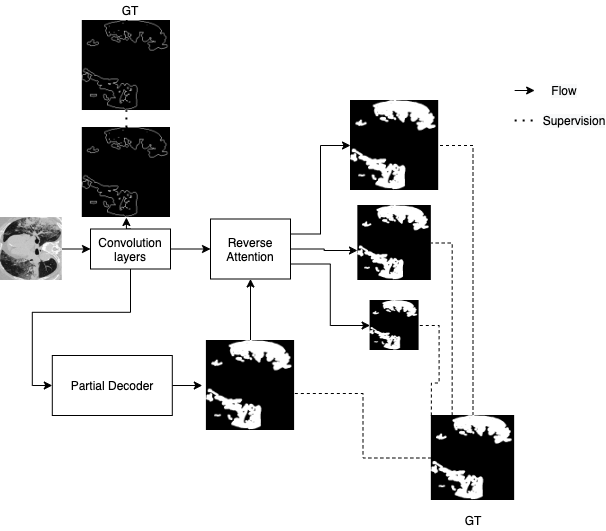
\includegraphics[width=88mm]{supervised-inf-net.png}
	\caption{Architecture of the supervised InfNet.  }
	\label{fig:supervised-inf-net_arch}
\end{figure}

\begin{figure*}
	\centering
	\small
	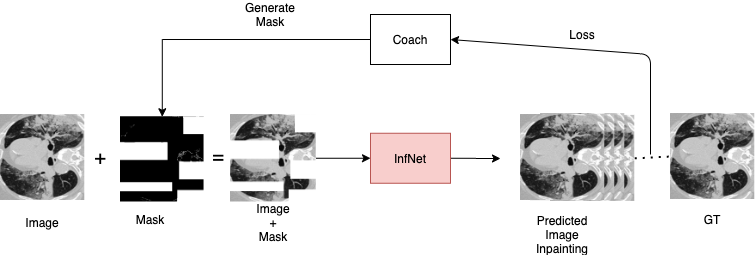
\includegraphics[width=\linewidth]{coach.png}
	\caption{The architecture of the coach network for self-supervised inpainting. }
\end{figure*}

\begin{figure*}
	\centering
	\small
	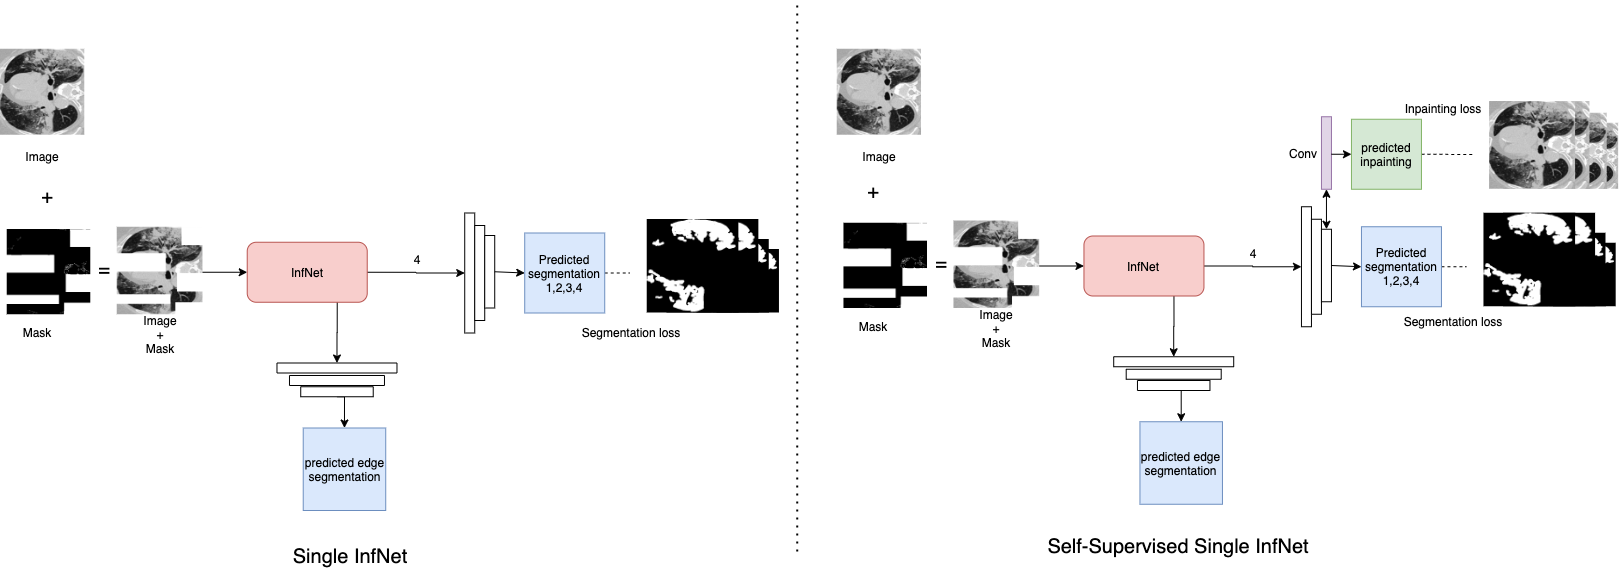
\includegraphics[width=\linewidth]{self-super-inf-net.png}
	\caption{The architecture of our self-supervised InfNet model. }
	\label{fig:inf-net_arch}
\end{figure*}

\begin{figure*}
	\centering
	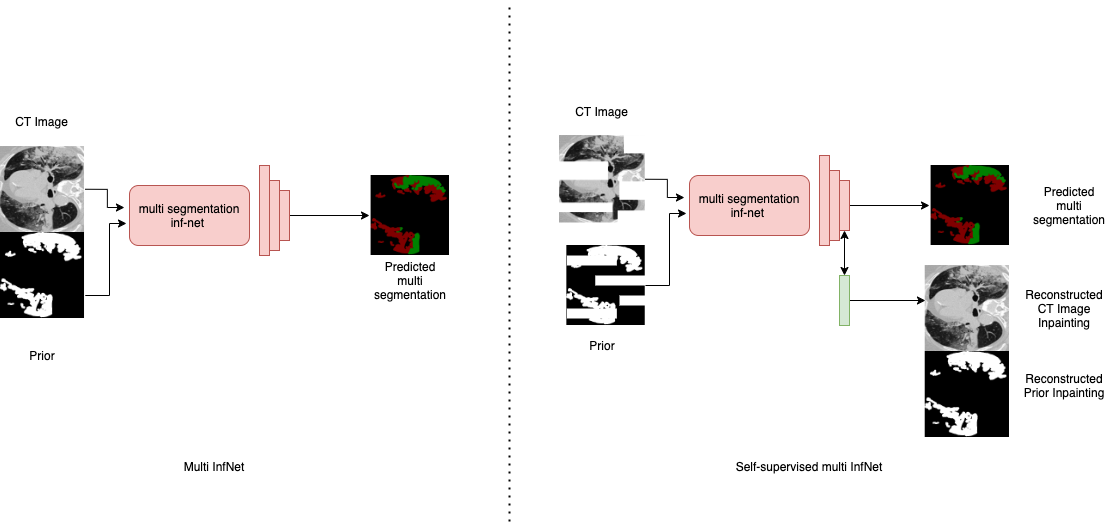
\includegraphics[width=\linewidth]{self-super-multi-inf-net.png}
	\caption{The architecture of our self-supervised multi segmentation InfNet model. Highlighted green block is the difference between the original multi InfNet and our self-supervised multi InfNet.}
	\label{fig:multi-inf-net_arch}
\end{figure*}



\subsection{Self-supervised InfNet for imaging segmentation}

We will propose using a self-supervised method to improve the performance of deep neural networks to create pixel-level segmentation for CT scan for lung images of COVID-19 patients. We will integrate self-supervised inpainting to pre-train our network. Since image inpainting is similarly related to image segmentation, we will integrate the pre-training steps as image inpainting for our image segmentation network. 

The original InfNet model would generate 5 different predictions: the edge segmentation prediction, and the other 4 are segmentation of the infected regions but of different sizes. In order to utilise the ability of self-supervised method for InfNet segmentation, we generate masks to be fed into the InfNet model. The last convolution layer that outputs the prediction is not used for the self-supervised case. However, the last convolutional layer is replace with a different convolutional layer to reconstruct the image and the edge appropriately. Everything else is kept the same as the InfNet architecture. This way the network will learn meaningful representations of the CT images and we can use these meaningful representations to learn the segmentation of the infected regions of the CT lung images. After learning the self-supervised features for InfNet, the training continues as normal similar to the InfNet algorithm. The training will start with the weights trained using the self-supervised inpainting method. The last layer will be changed to its original layer instead of the replaced convolutional layer. 

By learning features from image inpainting, the model can learn more features that are related to image segmentation. As creating mask can be a complex task for the network to learn to inpaint, the mask can either be too complex for the network to start learning or too simple to be able to learn good representations. We will be using a coach network that increases the complexity of the masking of the CT images throughout the training of the network. The mask created will initially be relatively simple, once the network is able to predict the inpainting of the CT images with good performance, the coach will increase the complexity of the masking to reduce the performance of the network, similar to how Generative Adversarial Network (GAN) works. The loss for the coach network is constructed from the loss of the image inpainting from the InfNet. The coach network and the InfNet both work together as a MinMax algorithm. The InfNet will try and minimize the loss to generate better image inpainting while the coach network will try to increase the loss of the image inpainting through generating more complex masks. In the beginning, the masks generated by the coach network will be less complex. Through training of the coach network, as the InfNet gets better at predicting image inpainting, the coach network generates a more complex masks. The loss fuction for the coach network is:
\begin{equation}
L_{coach}(x) = 1 - L_{rec}(x\odot M)
\end{equation}

where $M = C(x)$ which is created by the coach network. A constraint is apply to this loss function because the coach network would just create a mask that masks all region because no context information would be present for the network to learn and a maximum loss will be achieved. The constraint is:
\begin{equation}
\hat{B}(x) = B(x) - SORT(B(x))^{k|B(x)} 
\end{equation}
\begin{equation}
M = C(x) = \sigma (\alpha \hat{B}(x))
\end{equation}

The backbone, B, of the coach network has a similar network architecture with the model that inpaints the CT images. SORT(B(x)) sorts the features in descending order over the activation map. k represents the $k^{th}$ elements in the sorted list and k helps to control the fraction of the image to be erased. The region that has scores lesser than the $k^{th}$ element will be erased from the images. If k is 0.75 then 0.75 fraction of the images will not be erased. The score is scaled into a range of [0, 1] using a sigmoid activation function. We keep $\alpha = 1$ while training the coach network.

After the self-supervision training is finished, the single segmentation InfNet would reuse the self-supervised single InfNet network weights to train normally on the segmentation of the CT lung images. Likewise, the multi InfNet network would reuse the weights that were trained during self-supervised multi InfNet training to train normally on the segmentation of the CT lung images.

The proposed self-supervised single-labeled segmentation InfNet network architecture can be seen in \ref{fig:inf-net_arch}. The last layer for each output prediction is replace to a different linear activation layer. The linear activation layer will re-create the original image that is covered by the masks. 

The proposed self-supervised multi-labeled segmentation InfNet network architecture is shown in \ref{fig:multi-inf-net_arch}. The changes in the architecture for the multi-labeled segmentation InfNet is similar to the single-labeled segmentation InfNet where the last layer of the layer is replace with a different linear actiivation layer to output the inpainting of the original image. 


\begin{algorithm}
	\caption{Pseudo code for self-supervised with InfNet}
	\label{alg:self-inf-net}
	\begin{algorithmic}
		\STATE \textbf{Input:} $D_{labeled}$ = [($inputImage_1$, $G_{t1}$), ...]
		\FOR {each epoch}
		\FOR{each coach step}
		\STATE mask = M(x)
		\STATE maskedInput = $mask \odot inputImage$
		\STATE $ predictedImage =network(maskedInput), inputImage$
		\STATE $L_{rec} = CrossEntropy(predictedImage, inputImage)$
		\STATE $L_{coach}(x) = 1 - L_{rec}$
		\STATE update coach weights
		\ENDFOR
		\FOR {each network step}
		\STATE $P_{labeled} = Preprocess(D_{labeled})$ // data aug
		\STATE $inpaintingOutput = network(P_{labeled})$
		\STATE $L_{rec} = CrossEntropy(InpaintingOutput, inputImage)$
		\STATE backpropogate and save network weights
		\ENDFOR
		\ENDFOR 
		
		
		\FOR {each batch of $D_{labeled}$:}
		\STATE $P_{labeled}$ = Preprocess ($D_{labeled}$)
		\STATE $trainLoss = train(P_{labeled})$
		\STATE Backpropagate train loss
		\STATE $testLoss = test(P_{labeled})$
		\STATE save model weights, \textit{w}.
		\ENDFOR
	\end{algorithmic}
\end{algorithm}

We will also implement different data augmentation that includes random cropping, rotation, and random cutout to increase the number of available annotated data samples and labels as well as improve the model generalization as the data samples for CT images from COVID-19 can be limited. We will show that proper data augmentation affect the performance of the model by a marginal amount.

The output of the single segmentation InfNet will include the edge of the segmentation and four single-labeled segmentation of the infected region of the CT lung images with different sizes as shown in \ref{fig:supervised-inf-net_arch}. A loss will be calculated for each of the output from the single InfNet model. The first loss function is the loss edge, $L_{edge}$ which guides the model in representing better segmentation boundaries. The other loss function is the segmentation loss, ${L_{seg}}$. The segmentation loss combines both the loss of Intersection over Union (IoU) and the binary cross entropy loss. The segmentation loss equation for the single InfNet is as follows:
\begin{equation}
L_{seg} = L_{IoU} + \lambda L_{BCE}
\end{equation}

The $\lambda$ is set to 1 for this experiment. The segmentation loss is adapted to all of the ${S_i}$ predicted output where ${S_i}$ are created from $f_i$ such that $i={3,4,5}$. 

The total loss function for the single InfNet model is then:
\begin{equation}
L_{total} = L_{seg}(G_t, S_g) + L_{edge} + 	\sum_{i=3}^{5}L_{seg}(G_t, S_i)
\end{equation}

The summation of the loss functions are calculated from the output of the three convolutional layers. $G_t$ refers to the ground truth labels. $S_g$ is the output from the parallel partial decoder to match with the ground truth label.

As for the multiple segmentation infected region InfNet. We also use the default model and hypermaters from the InfNet code. We will however train the network without using any unlabeled images to be used as a supervised version. The CT lung images and prior (infected region) for the CT lung images are concatenate together before being fed into the multiple segmentation InfNet. The prior is generated from the single segmentation InfNet. The prior would contain the area of the infected region. However, the prior does not contain the labels for ground-glass opacities and consolidations. It just shows the infected regions. The multiple segmentation InfNet will label the CT lung images with background, ground-glass opacities, and consolidations. The architecture for multiple segmentation InfNet can be seen in \ref{fig:multi-inf-net_arch}. The loss function for the multiple segmentation InfNet is as follow:
\begin{equation}
L_{bce} = \frac{1}{N}\sum_{i=1}^{N} y_i \cdot log(\hat{y_i}) + (1-y_i)\cdot log(1-\hat{y_i})
\end{equation}

The loss function for multiple segmentation InfNet uses the binary cross-entropy between the predicted segmentation and the ground truth segmentation.

In order to improve the performance of the model and to aid in the generalisation, we  determine to use self-supervised learning to learn good representations of the CT scan of lung images. Self-supervised learning generates auxiliary tasks from the labeled data samples. For instance, when undergoing data augmentation with rotation, we could train the network to predict if the images have been rotated 0 degree, 90 degree, 180 degree to learn representations of the images. 


\subsection{Estimation of Severity of COVID-19 from CT images}
Once the network is able to predict the pixel-level segmentation of the CT scan images, we will use the pre-trained network to predict the segmentation of the infected region. We will then calculate the ratio between the segmentation of the infected region and the segmentation of the parenchyma in the ICTCF dataset. We use the algorithm provided by ICTCF to split the parenchyma from the CT lung images. We manually remove images that the parenchyma were not splitted properly. There were 6654 images from 1338 patients. After cleaning the dataset, we ended up with 6613 CT lung images with properly splitted parenchyma. We will then calculate the ratio between the infected lung region predicted by our network with the splitted parenchyma from the CT lung images to determine the severity of the lung. The CT lung images is first fed into the single SInfNet networks to generate the infected region. The infected region will have the shape of the CT lung images. Each pixel of the predicted infected region represent the amount of infection that range from 0 to 1 where 0 is not infected and 1 is highly infected. We will add the sum of the predicted infected region and divide it by the area of the parenchyma to obtain the ratio. The higher the ratio between the infected region and the splitted parenchyma, the higher the severity of the lung.

%determine the severity score of the lung regions through several methods. The severity score of the lungs can be determined by using CT severity score (CT-SS) \cite{ref11}. The score uses lung opacification for extension of the infections in the lungs. CT-SS is an adaptation from the method previously used in patients after severe-acute respiratory syndrome (SARS) \cite{ref10} to describe ground-glass opacity, interstitial opacity, and air trapping. The lungs will be divided into 20 regions, the posterior apical segment of upper left lobe was divided into apical and posterior segmental regions, the anteromedial basal segment of lower left lobe will be divided into anterior and basal segmental regions. For each region, there contain a system attributing scores of 0, 1, 2, either parenchymal opacification involves 0%, less than 50%, or equal to or more than 50%. The CT-SS will calculate the sum of individual scored regions. The final value of CT-SS can range from 0 to 40.

The equation for the ratio calculation is as follows:

\begin{equation}
Ratio = \frac{\hat{y}}{P}
\end{equation}

Where $P$ refers to the area of the parenchyma region and $\hat{y}$ refers to the automatically segmented infected regions by the network.

We will compare our method against supervised and semi-supervised \cite{ref13,ref14} models trained on COVID-19 dataset. For comparing supervised learning, we will compare against the paper \cite{ref13}. We will train and follow using the same network structure but change from supervised learning to self-supervised learning and compare the performance between supervised and self-supervised.

When comparing with the semi-supervised model, we determine that our model is successful if our model is able to reach close to or better than the performance of the semi-supervised model as semi-supervised model is able to obtain a higher amount of data samples by looking at both unannotated and annotated data samples while self-supervised model only have access to the annotated labels. A self-supervised learning method will create its own training annotated labels without any manual human labelling and trained without any unlabeled data samples. We will compare our method’s performance against InfNet \cite{ref14} which uses semi-supervised learning by generating pseudo labels from randomly selected unlabeled CT images.

Our method will be novel compare to the other methods mentioned as our method will be integrating both the segmentation of the CT lung images as well as the calculation of the severity score through caluclation of the segmented infected lung areas.



\iffalse
The pseudo-code for the training of baseline model is relatively straightforward as can be seen in \ref{alg:baseline}.
\begin{algorithm}
	\caption{Pseudo code for InfNet}
	\label{alg:baseline}
	\begin{algorithmic}
		\STATE \textbf{Input:} Train data $D_{labeled}$,  test data $D_{t-labeled}$ ground truth $G_t$,
		\FOR {each batch of $D_{labeled}$:}
		\STATE $P_{labeled}$ = Preprocess $D_{labeled}$
		\STATE $L_{seg}(G_t, S_g), L_{edge}, L_{seg}(G_t, S_3), L_{seg}(G_t, S_4), L_{seg}(G_t, S_5)	$  = train(\textit{M},  $P_{labeled}$)
		\STATE $L_{traintotal} = L_{seg}(G_t, S_g) + L_{edge} + L_{seg}(G_t, S_3) + L_{seg}(G_t, S_4) + L_{seg}(G_t, S_5)$
		\STATE plot($L_{traintotal}$)
		\STATE = test(\textit{M}, $D_{t-labeled}$)
		\STATE plot(test loss)
		\STATE save model weights, \textit{w}.
		\ENDFOR
	\end{algorithmic}
\end{algorithm}
\fi 
\section{Experiments}

\subsection{Datasets}
The dataset that we will be using is an integrative resource of chest computed tomography images and clinical features of patients with COVID-19 pneumonia (ICTCF) \cite{ref23} which contains the severity score for each CT lung image. ICTCF contains 127 types of clinical features and laboratory confirmed cases of COVID-19 from 1170 patients. The dataset can be found here: http://ictcf.biocuckoo.cn/ . 

The datasets that we will be using to compare with for the segmentation results will be the datasets from Inf-Net\cite{ref14} and the datasets from medseg\cite{ref26}. The dataset from Inf-Net\cite{ref14} contains 68 labeled CT images while the dataset from medseg contains 911 labeled CT images. In total, the number of labeled segmented CT images is 979.

The other datasets that we will be focusing on are COVID-CT-Dataset \cite{ref21} and covid-chestxray-dataset \cite{ref22}. COVID-CT-Dataset can be found at https://github.com/UCSD-AI4H/COVID-CT. COVID-CT-Dataset consist of 349 CT images obtianed from 216 patients. Covid-chestxray-dataset can be found at https://github.com/ieee8023/covid-chestxray-dataset. COVID-CT-Dataset  was created through assembling medical images from publications and websites and contains 123 frontal view X-rays of the lungs. An additional dataset that we can use is from Cell \cite{ref24}, http://ncov-ai.big.ac.cn/download?lang=en if we have enough capacity to load the dataset as the dataset can be huge. This dataset is constructed from the China Consortium of Chest CT Image investigation (CC-CCII). The CT images are classified into novel coronavirus pneumonia (NCP) caused by SARS-CoV-2 virus, common pneumonia and normal controls. It consists of 617,775 CT images obtained from 4,154 patients.

\subsection{Data Augmentation}
We used data augmentation to increase our data samples size. The data agumentation that we used includes \textit{vertical flipping, horizontal flipping, random crop, and random cutout}. For the random cutout percentage, we experimented that 0.5 cutout of the CT lung images yield higher performance than the rest of the value. This is because entropy at 0.5 is the highest which could increase more variability of the images. Examples of the data augmentation can be seen in figure \ref{fig:data_aug}.

\begin{figure}
	\centering
	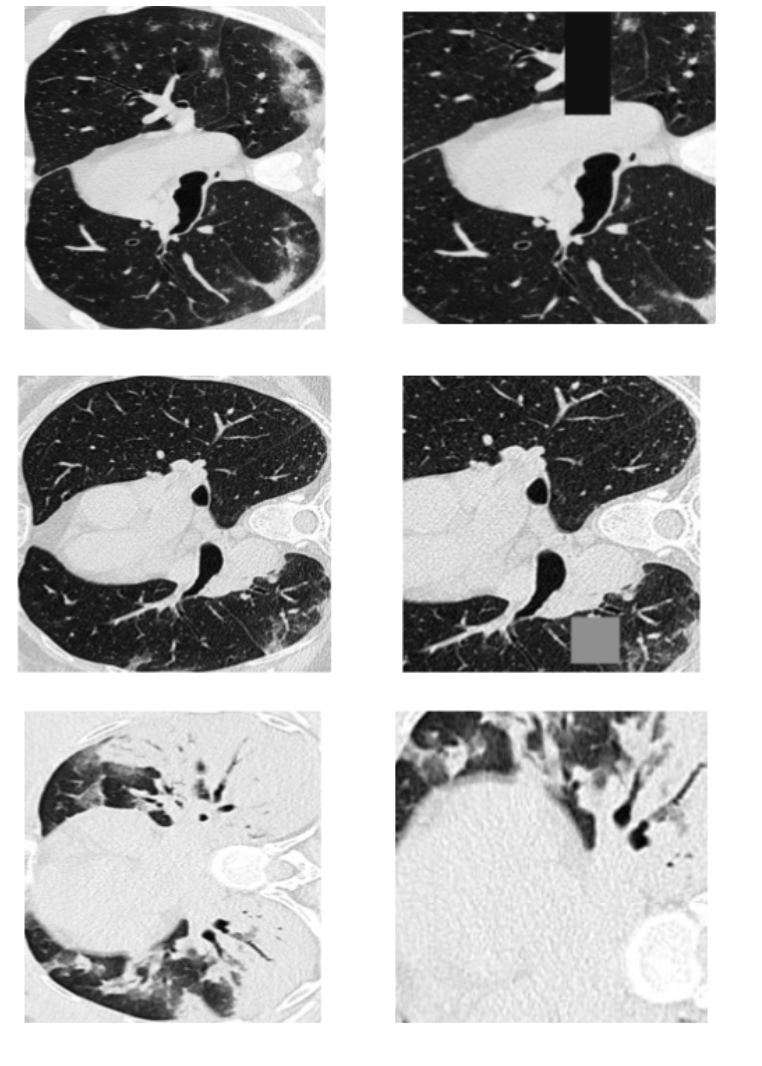
\includegraphics[width=\linewidth]{data_aug.png}
	\caption{Example CT lung images of our data augmentation. The left column is the original CT lung images while the right column is the augmented CT lung images. The first row of the CT lung images involves random cropping and random cutout. The second row of the CT lung images involves random cropping and random cutout. The third row of the CT lung images involves random cropping and vertical flipping. We can see the random cutout involves patching the image with colors of the same value of rgb. For instance, if the value of r is 10, then the value of g and b are also 10. If the value of r is 50, then the value of g and b are also 50.}
	\label{fig:data_aug}
\end{figure}

\subsection{Performance evaluation of image segmentation}
We have trained the supervised inf-net as baseline with comparison to the supervised inf-net with additional data augmentation. The comparison for the methods can be seen in \ref{tab:table_compare}. We can see that the additional data augmentation improves the performance of the baseline model. For the single segmentation Inf-Net comparison, we can see the performance of the single segmentation Inf-Net improves the most when the random cutout is set to a value of 0.5 without any self-supervised training. 

However, the loss calculation does not truly evaluate the performance of the model. We use an additional performance metrics to calculate the model performance. The performance metrics we will be using is called dice similarity coefficient. As shown in \ref{tab:dice_compare}, we see that the best performing model is the self-supervised single Inf-Net using the dice similarity coefficient. 

\subsection{severity estimation results}


\begin{table}
	\centering

	\begin{tabular}{|l|l|l|}
		\hline
		& single Inf-Net & multi Inf-Net \\\hline
		SInfNet & \textbf{0.60} & 0.93  \\\hline
		SInfNet+data aug (0.4)& 0.67 & 2.74  \\\hline
		SInfNet+data aug (0.5)& 0.65 & \textbf{} \\\hline
		Self-super & 0.67 & \\\hline
		Self-super+data aug & 0.71 & \\
		\hline
		
	\end{tabular}
	\caption{Comparison of supervised inf-net (SInf-Net) model with added data augmentation. The values listed in the table represent the test loss. The floating value  after the data augmentation refers to the fraction of the image randomly cutout. 0.2 shows that 0.2 of the image is cutout to be empty. }
	\label{tab:table_compare}
\end{table}

\begin{table}
	\centering
	
	\begin{tabular}{|l|l|l|}
		\hline
		& single Inf-Net & multi Inf-Net \\\hline
		SInfNet &  0.26 & 0.12  \\\hline
		SInfNet+data aug (0.4)&  0.31 & 0.66  \\\hline
		SInfNet+data aug (0.5)& 0.30 & \textbf{} \\\hline
		Self-super & 0.31  & \\\hline
		Self-super+data aug & \textbf{0.34} & \\
		\hline
		
	\end{tabular}
	\caption{Comparison of supervised inf-net (SInf-Net) model with added data augmentation. The values listed in the table represent the  dice similarity coefficient. The floating value  after the data augmentation refers to the fraction of the image randomly cutout. 0.2 shows that 0.2 of the image is cutout to be empty. }
	\label{tab:dice_compare}
\end{table}

\iffalse
\begin{table*}[t]
	\centering
	\small
	\begin{tabular}{|l|l|}
		\hline
		Sub-Tasks & Time  \\\hline
		Research on related self-supervised tasks to incorporate the methods into COVID-19 pixel-level image segmentation & 1 week  \\\hline
		Find related COVID-19 dataset for classification labels(for self-supervised) and pixel-level segmentation(for classification) labels & 1 week  \\\hline
		Find baseline methods to compare against & 2 week  \\\hline
		Implement self-supervised method for pixel-level segmentation on COVID-19 segmentation & 3 week  \\\hline
		Experiment and training (including calculating the severity score for lung regions) & 3 week  \\\hline
		Write and finalize paper if successful & 2 week  \\\hline
		
	\end{tabular}
	\caption{Tasks scheduled}
	\label{tab:2}
\end{table*}
\fi

\section{Result}
In this section, we show the results of our experiments obtained. To evaluate the performance of our proposed self-supervised InfNet, we compare its performance with other state-of-the-art methods including the original InfNet.

\subsection{Result comparison for Single InfNet}
Table \ref{tab:single} shows the result for the single segmentation InfNet. The single segmentation InfNet does not segment between ground-glass opacities or consolidation. The single segmentation segments and represents all infected region as one. We can see that self-supervision can improve on the generalization and consistency in predicting the different CT lung images as they perform the best in terms of the error range. Even though the baseline single InfNet (Single SInfNet) performance has better mean values for F1, IoU, and Recall, the self-supervised approach helps to create robustness and consistency in the model itself to better handle outliers. We can see the results of the single segmentation in Figure \ref{fig:single-comparison}. We can see that the baseline single InfNet (Single SInfNet) overestimated the infected region of an outlier in the segmentation result in the figure in the last row. The self-supervised Single InfNet (Single SSInfNet) did a better job at predicting outliers where its prediction is more closely related to the ground truth than the baseline single SInfNet. The receiving operating characteristics (ROC) can be seen in Figure \ref{fig:single_rocs}. The baseline Single InfNet (Single SInfNet) has the best performing ROC when compared to the other networks.
 
  \begin{figure*}
 	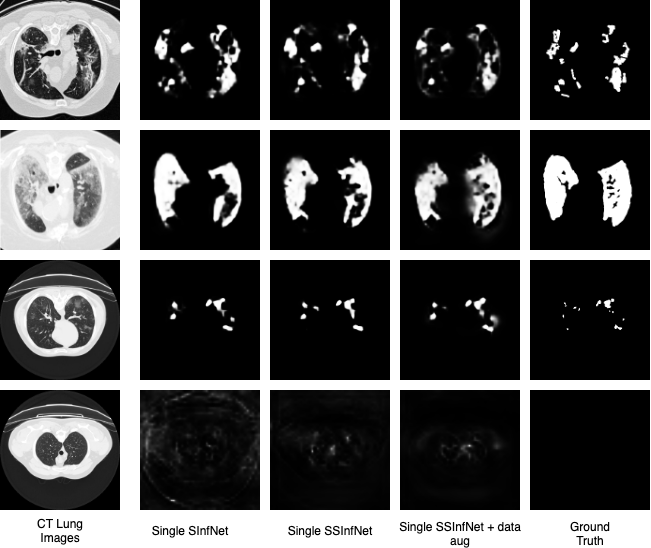
\includegraphics[width=\linewidth]{comparison_single.png}
 	\caption{Comparison of single segmentation between different networks. Overall, the Single SInfNet achieves a better performance than the rest of the network as seen in row 1 to row 3. However, our method by adding self-supervised to InfNet (Single SSInfNet) prevents overestimating the infected region of the CT lung images as can be seen in row 4.}
 	\label{fig:single-comparison}
 \end{figure*}

 \begin{figure*}
 	\centering
 	\small
 	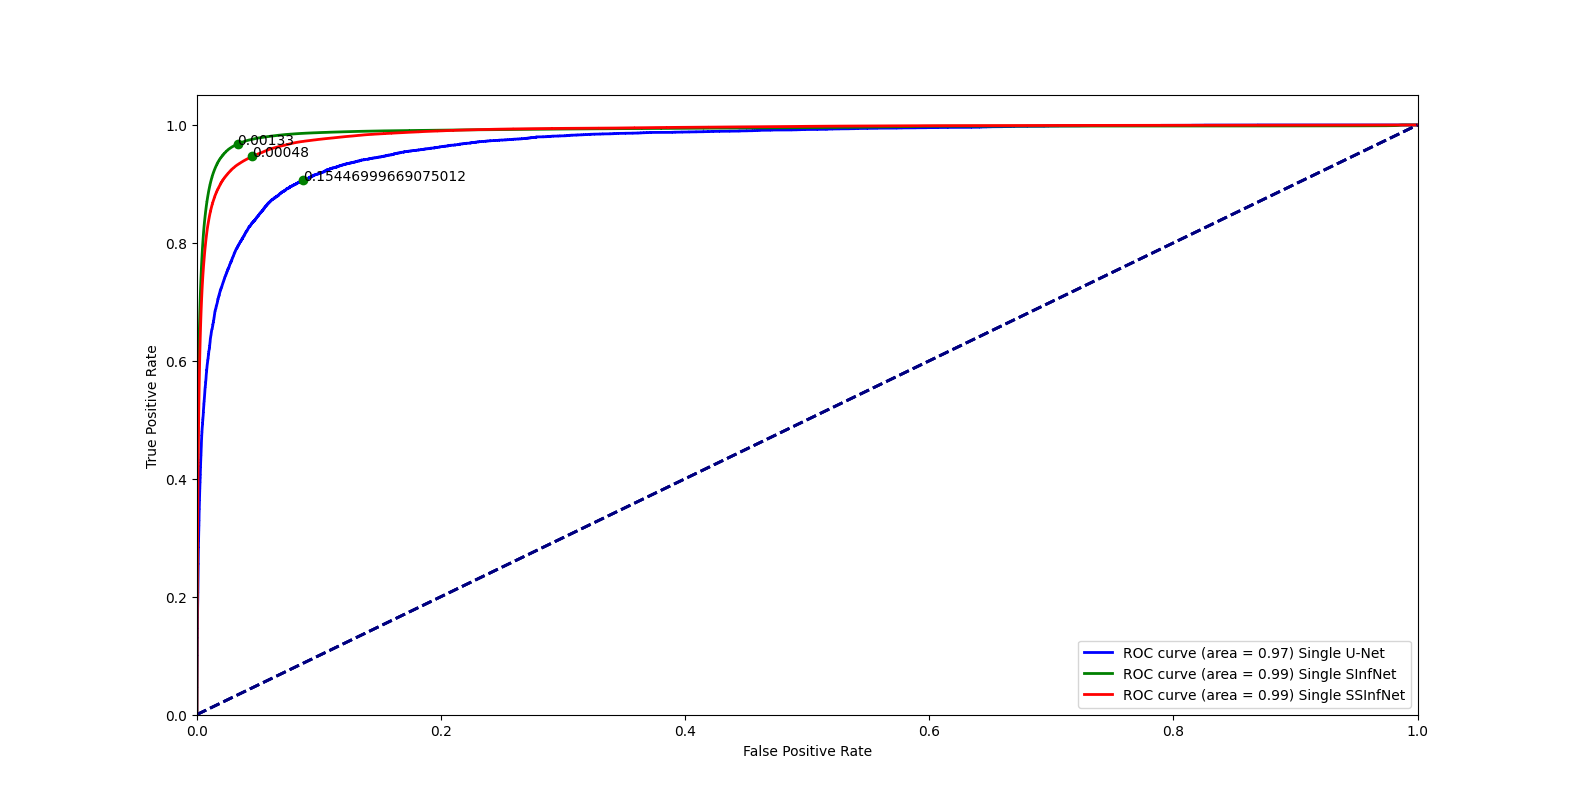
\includegraphics[width=\linewidth]{single_rocs.png}
 	\caption{ROC comparison of different networks.}
 	\label{fig:single_rocs}
 \end{figure*}
 
 \begin{table*}[!ht]
 	\centering
 	\begin{tabular}{| c | c || c c c c c ||}
 		\hline
 		Methods & & F1 & IoU & Recall & Precision & AUC \\ \hline
 		Single SInfNet &  Mean & \textbf{0.39} & \textbf{0.29} & \textbf{0.83} & 0.33 & \textbf{0.9909} \\ \cline{2-7}
 		& Error & $\pm$ 0.059 & $\pm$ 0.053 & $\pm$ \textbf{0.069} & $\pm$0.057  & $\pm$0.032 \\ \hline
 		Single SSInfNet &  Mean & 0.38 & 0.27 & 0.75 & 0.33 & 0.9883  \\ \cline{2-7}
 		& Error & $\pm$0.056 & $\pm$0.049 &$\pm$0.077  & $\pm$0.053 & $\pm$  0.010 \\ \hline
 		Single SSInfNet + data aug &  Mean & 0.30 & 0.20 & 0.72 & 0.28 &  0.9795 \\ \cline{2-7}
 		& Error & $\pm$ \textbf{0.050}  & $\pm$  \textbf{0.039} & $\pm$ 0.085 & $\pm$\textbf{0.045} & $\pm$ \textbf{0.006}  \\ \hline
 	\end{tabular}
 	\caption{Quantitative result for comparison between Single segmentation InfNet and self-supervised single segmentation InfNet in the test set. Single SSInfNet is our self-supervised single InfNet.}
 	\label{tab:single}
 \end{table*}


\subsection{Results comparison for Multi InfNet}
Table \ref{tab:multi-weakprior} shows the result for the comparison between multiple segmentation InfNet. As the multiple segmentation InfNet requires a CT lung image concatenate with a prior as input where the prior is the segmentation of the infected region of the CT lung without considering the location of ground-glass opacities or consolidation. The prior represents the infected region as a whole. The prior is obtained by running prediction of the infected region by the single segmentation InfNet on the CT lung images of the test set. Then the prior is fed together with the CT lung image from the test set into the multiple segmentation InfNet to obtain the result. As the baseline Single InfNet achieves the best performing single InfNet, we use the prediction of the prior obtained from the baseline Single InfNet to be fed into the multi segmentation InfNet with the CT lung images. The self-supervised Multi InfNet (SSInfNet) was able to achieve a higher performance than the baseline Multi InfNet (SInfNet). The self-supervised Multi InfNet (SSInfNet) achieves the best performance in evaluating the ground-glass opacities and the consolidation area of the CT lung images than the baseline Multi InfNet (SInfNet). In order to further improve our self-supervised Multi InfNet (SSInfNet), we added focal loss and lookahead optimizer. The improvement of the self-supervised Multi InfNet (SSInfNet) improved and has the highest performance comparing to the other networks. The overall performance of the self-supervised Multi InfNet (SSInfNet) with added focal loss and lookahead optimizer achieves the best result. We can see the segmentation result in Figure \ref{fig:multi-weakprior-comparison}. However, the baseline Multi InfNet (SInfNet) achieves a better recall score than the rest of the networks. As we can see in Figure \ref{fig:multi-weakprior-comparison}, the baseline multi InfNet (SInfNet) predicted more of the consolidation even on areas that is not infected. On the third row, the SInfNetoverestimated the consolidation area in the healthy CT lung image. As recall is the amount of true positive over the total actual consolidation area, the SInfNet seems to over-predict the consolidation area which results in a higher recall score than the other networks. However, as the prediction of the consolidation area for the baseline Multi InfNet is not accurate, the precision for the baseline Multi InfNet is lower. This causes the SInfNet to have a lower performance than our SSInfNet method.
 
 \begin{table*}[!h]
 	\centering
 	\small
 	\begin{tabular}{| c | c || c c c c || c c c c |}
 		\hline
 		& &\multicolumn{4}{c||}{Ground-Glass Opacity} & \multicolumn{4}{c|}{Consolidation}\\ \cline{3-10}
 		Methods & & F1 & IoU & Recall & Precision & F1 & IoU & Recall & Precision \\\hline
 		U-Net & Mean & 0.26 & 0.18 & 0.216 & 0.405 & 0.35 & 0.26 & 0.32 & 0.46 \\ \cline{2-10}
 		& Error & $\pm$0.057 & $\pm$0.043 & $\pm$0.053 & $\pm$0.085 & $\pm$0.097 & $\pm$0.08 & $\pm$0.089 & $\pm$0.116  \\ \hline
 		SInfNet & Mean & 0.38 & 0.27 & \textbf{0.58} & 0.41 & 0.29 & 0.22 & \textbf{0.61} & 0.31  \\ \cline{2-10}
 		& Error & $\pm$0.054 & $\pm$0.042 & $\pm$0.065 & $\pm$0.058 & $\pm$0.078 & $\pm$0.068 & $\pm$0.099 & $\pm$0.084  \\ \hline \hline
 		
 		\vtop{\hbox{\strut SSInfNet}\hbox{\strut }} & Mean & 0.36 & 0.26 & 0.56 & 0.4 & 0.31 & 0.25 & 0.56 & 0.38 \\ \cline{2-10}
 		& Error & $\pm$0.055 & $\pm$0.043 & $\pm$0.067 & $\pm$0.059 & $\pm$0.087 & $\pm$0.076 & $\pm$0.114 & $\pm$0.097 \\ \hline \hline
 		
 		\vtop{\hbox{\strut SSInfNet+}\hbox{\strut focal loss+}\hbox{\strut lookahead}} & Mean & \textbf{0.43} & \textbf{0.31} & \textbf{0.58} & \textbf{0.48} & \textbf{0.46} & \textbf{0.36} & 0.56 & \textbf{0.56} \\ \cline{2-10}
 		& Error & $\pm$0.057 & $\pm$0.046 & $\pm$0.072 & $\pm$0.059 & $\pm$0.096 & $\pm$0.088 & $\pm$0.11 & $\pm$0.101 \\ \hline \hline \hline
 		
 		
 		& &\multicolumn{4}{c||}{Background} & \multicolumn{4}{c|}{Overall}\\ \cline{3-10}
 		Methods & & F1 & IoU & Recall & Precision & F1 & IoU & Recall & Precision \\\hline
 		U-Net & Mean & 0.857 & 0.754 & 0.998 & 0.755 &  0.49 & 0.40 & 0.51 & 0.54  \\ \cline{2-10}
 		& Error &  $\pm$ 0.01 & $\pm$0.017 & $\pm$0.001 & $\pm$0.017 & $\pm$ 0.055 & $\pm$0.046 & $\pm$0.048 & $\pm$0.073 \\ \hline
 		SInfNet & Mean & 1.0 & 0.99 & 0.99 & 1.0 & 0.55 & 0.5 & \textbf{0.73} & 0.57   \\ \cline{2-10}
 		& Error & $\pm$0.002 & $\pm$0.003 & $\pm$0.002 & $\pm$0.002 & $\pm$0.044 & $\pm$0.038 & $\pm$0.055 & $\pm$0.048 \\ \hline
 		\vtop{\hbox{\strut SSInfNet}\hbox{\strut }} & Mean & 1.0 & 0.99 & 1.0 & 1.0 & 0.56 & 0.5 & 0.71 & 0.59 \\ \cline{2-10}
 		& Error & $\pm$0.002 & $\pm$0.003 & $\pm$0.002 & $\pm$0.002 & $\pm$0.048 & $\pm$0.041 & $\pm$0.061 & $\pm$0.053\\ \hline \hline

 		\vtop{\hbox{\strut SSInfNet+}\hbox{\strut focal loss+}\hbox{\strut lookahead}} & Mean &1.0 & 0.99 & 0.99 & 1.0 & \textbf{0.63} & \textbf{0.55} & 0.71 & \textbf{0.68} \\ \cline{2-10}
 		& Error & $\pm$0.002 & $\pm$0.003 & $\pm$0.002 & $\pm$0.002 & $\pm$0.052 & $\pm$0.046 & $\pm$0.061 & $\pm$0.054\\ \hline \hline \hline
 		
 	\end{tabular}
 	\caption{Quantitative result of Ground-glass Opacities \& Consolidation on the test data set. Prior is obtained from the single segmentation InfNet. SSInfNet is our self-supervised multi InfNet. }
 	\label{tab:multi-weakprior}
 \end{table*}

  \begin{figure*}
 	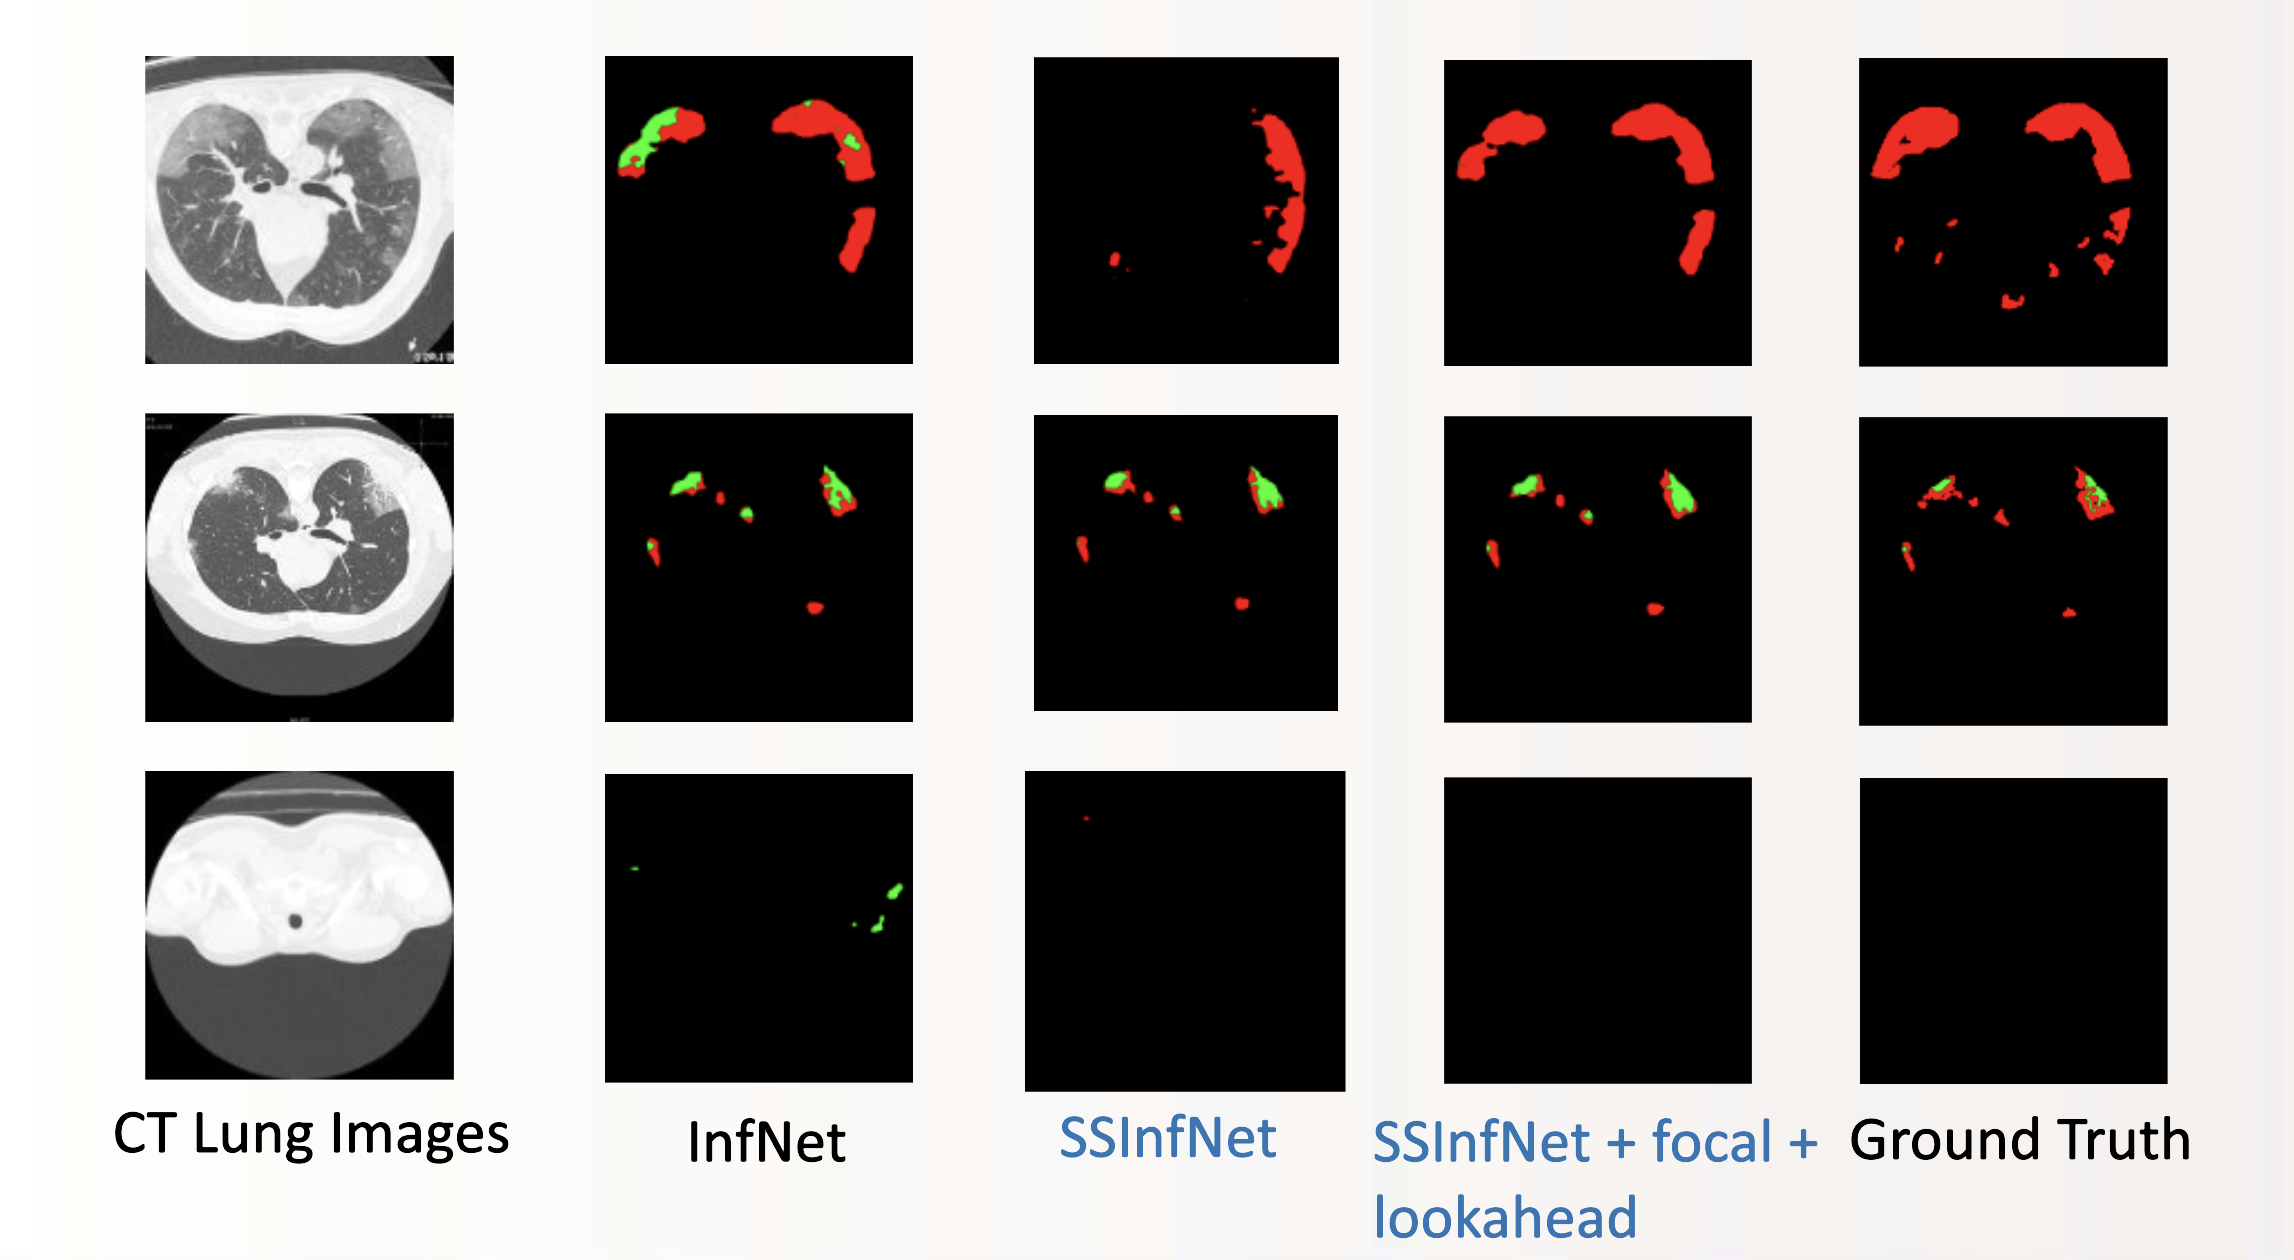
\includegraphics[width=\linewidth]{comparison_multi_weakprior.png}
 	\caption{Comparison of multi segmentation between different networks with prior generated from single InfNet. Red colored is the ground-glass opacities and green colored is the consolidation. The baseline multi InfNet overestimated the consolidation region in the first and third row of the CT lung image when there are not suppose to be any consolidation region.}
 	\label{fig:multi-weakprior-comparison}
 \end{figure*}

\section{Conclusion}
Our results show that the integration of self-supervised image in-painting to the supervised multi segmentation InfNet improves the performance of both the ground-glass opacities and the consolidation in the dataset that we used. Additionally, adding focal loss and lookahead optimizer further improves our self-supervised multi InfNet and achieves 0.63 F1 scores. The improvement in the performance of the infected region segmentation for ground-glass opacities and consolidation of CT lung images can help prevent negatively assessing that a patient contains irregular patterns when the patients are healthy. This would prevent patients from receiving unnecessary treatments that could cause side effects. For the future work, we could apply this technique for other datasets that include segmenting Leukemia or breast cancer images.

\section*{Acknowledgment}
I would like to acknowledge Dr. PingZhao Hu and Dr. Carson Leung for the supervision of this Honours Project. I have learned a lot about the technique and best practices to write a good paper. I would like to thank Judah Zammit and Qian Liu too, they have recommended me several methods and tools to improve on the work for this project. I would also like to acknowledge Dr. Ruppa Thulasiram for the opportunity to be able to take this course with Dr. PingZhao Hu and Dr. Carson Leung as my supervisor. I would not be able to get this much opportunity and learned all these without them. I would like to add ICTCF and MedSeg as an acknowledgement for providing the publicly available COVID-19 CT lung images dataset. The publicly available dataset has helped us been able to carry out this research.
\begin{thebibliography}{1}
	%\textit{Basic Format for Books:}\\
	
	\bibitem{ref1}Krizhevsky, A, Sutskever, I. , and Hinton G. \textit{Imagenet classification with deep convolutional neural networks.} In NIPS, 2012.
	
	\bibitem{ref2} Fan, DP., Zhou, T., Ji, GP., et al. \textit{Inf-Net: Automatic COVID-19 Lung Infection Segmentation from CT Scans.} arXiv preprint arXiv:2004.14133v2, 2020.
	
	\bibitem{ref3} Alom, MZ., Rahman, MMS., Nasrin, MS., Taha, TM., Asari, VK. \textit{COVID-MTNet: COVID-19 Detection with Multi-Task Deep Learning Approaches.} arXiv:2004.03747, 2020.
	
	\bibitem{ref4} Yan, Q., Wang, B., Gong, D., et al. \textit{COVID-19 Chest CT Image Segmentation -- A Deep Convolutional Neural Network Solution.} arXiv:2004.10987, 2020.
	
	\bibitem{ref5} Ronneberger, O., Fischer, P., and Brox, T. \textit{U-net: Convolutional networks for biomedical image segmentation.} In MICCAI, pages 234–241. Springer, 2015. 2
	
	\bibitem{ref6} Khobahi, S., Agarwal, C., Soltanalian, M. \textit{CoroNet: A Deep Network Architecture for
		SemiSupervised Task-Based Identification of COVID-19 from Chest X-ray Images.} In medRxiv, 2020.
	
	\bibitem{ref7} Cohen, J. P., Dao, L., Morrison, P., Roth, K., Bengio, Y., Shen, B., Abbasi, A., Hoshmand-Kochi, M., Ghassemi, M., Li, H., Duong, T. Q. \textit{Predicting covid19 pneumonia severity on chest x-ray with deep learning}, arXiv preprint arXiv:2005.11856.
	
	\bibitem{ref8} Lin, TY., Goyal, P., Girshick, R., He, K., and Dollar, P. \textit{Focal loss for dense object detection.} arXiv preprint arXiv:1708.02002, 2017
	
	\bibitem{ref9} Duchi, J., Hazan, E., and Singer, Y. \textit{Adaptive subgradient methods for online learning and stochastic optimization.} Journal of Machine Learning Research, 12(Jul):2121–2159, 2011.
	
	\bibitem{ref10} Kingma, D.P., and Ba, J. \textit{Adam: A method for stochastic optimization.} arXiv preprint arXiv:1412.6980, 2014.
	
	\bibitem{ref11}  Zhang, M.R., Lucas, J., Hinton, G., and Ba, J. \textit{Lookahead optimizer: k steps forward, 1 step back.} arXiv preprint arXiv:1907.08610, 2019.
	
	\bibitem{ref12} Ning, Lei, WS., Yang SJ., et al. (2020). \textit{iCTCF: an integrative resource of chest computed tomography images and clinical features of patients with COVID-19 pneumonia.} 10.21203/rs.3.rs-21834/v1.
	
	\bibitem{ref13} \textit{COVID-19 CT segmentation dataset}. Retrieved from http://medicalsegmentation.com/covid19/.
	
	\bibitem{ref14} Yan, Q., Wang, B., Gong D., et al. \textit{COVID-19 Chest CT Image Segmentation – A Deep Convolutional Neural Network Solution.} arXiv preprint arXiv:2004.10987, 2020.

	
	\bibitem{ref15} Kalluri, T., Varma, G., Chandraker, M., and Jawahar, CW. \textit{Universal semi-supervised semantic segmentation.} CoRR, abs/1811.10323, 2018.
	
	\bibitem{ref16} Misra, I., and van der Maaten, L.\textit{ Self-supervised learning of pretext-invariant representations.} arXiv preprint arXiv:1912.01991, 2019.
	
	\bibitem{ref17} Chen, T., Kornblith, S., Norouzi, M., and Hinton, G. \textit{A simple framework for contrastive learning of visual representations.} arXiv:2002.05709, 2020.
	
	\bibitem{ref18} Newell, A., Deng, J. \textit{How Useful is Self-Supervised Pretraining for Visual Tasks?} arXiv:2003.14323, 2020.
	
	\bibitem{ref19} Novosel, J., Viswanath, P., and Arsenali, B. \textit{Boosting Semantic Segmentation With Multi-Task Self-Supervised Learning for Autonomous Driving Applications.} In Proc. of NeurIPS - Workshops, pages 1–11, Vancouver, BC, Canada, Dec. 2019.
	
	\bibitem{ref20} Kahl, F. \textit{“Fine-grained segmentation networks: Self-supervised segmentation for improved long-term visual localization,”} in Proceedings of the IEEE International Conference on Computer Vision, 2019, pp. 31–41.
	
	\bibitem{ref21} Chang, YC., Yu, CJ., Chang, SC., et al. \textit{Pulmonary sequelae in convalescent patients after severe acute respiratory syndrome: evaluation with thin-section CT.} Radiology 2005; 236(3):1067-1075.
	
	\bibitem{ref22} Yang, R., Li, X., Liu, H., Zhen, Y., Zhang, X., Xiong, Q., et al. \textit{Chest CT Severity Score: An Imaging Tool for Assessing Severe COVID-19. Radiol Cardiothorac Imaging.} 2020;2(2):e200047.
	
	\bibitem{ref23} Shan, F., Gao, Y., Wang, J., Shi, W., Shi, N., Han, M., Xue, Z., and Shi, Y. \textit{Lung Infection Quantification of COVID-19 in CT Images with Deep Learning.} arXiv preprint arXiv:2003.04655, 1-19, 2020.

	

	

	\bibitem{ref24} Kolesnikov, A., Zhai, XH., and Beyer, L. \textit{Revisiting self-supervised visual representation learning.} In Conference on Computer Vision and Pattern Recognition (CVPR), 2019.

	\bibitem{ref25} Trinh, TH., Luong, MT., and Le, QV. \textit{Selfie: Self-supervised pretraining for image	embedding.} arXiv preprint arXiv:1906.02940, 2019.

	\bibitem{ref26} Frinken, V., Zamora-Martinez, F., Espana-Boquera, S., Castro-Bleda, M. J., Fischer, A., and Bunke, H. (2012). \textit{Long-short term memory neural networks language modeling for handwriting recognition.} In Pattern Recognition (ICPR), 2012 21st International Conference on, pages 701–704. IEEE.

	\bibitem{ref27}  LeCun, Y., Haffner, P., Bottou, L., and Bengio, Y. \textit{Object recognition with gradient-based learning.} In Shape, contour and grouping in computer vision, pages 319–345. 1999.

	\bibitem{ref28} Kingma, DP. and Welling, M. \textit{Auto-Encoding Variational Bayes.} In The 2nd International Conference on Learning Representations (ICLR), 2013.

	\bibitem{ref29}  Goodfellow IJ., Pouget-Abadie, J., Mirza, M., Xu, B., Warde-Farley, D., Ozair, S., Courville, AC., and Bengio, Y. \textit{Generative adversarial nets.} In Proceedings of NIPS, pages 2672– 2680, 2014.

	\bibitem{ref30} Zhao, JY., Zhang, YC., He, XH., Xie, PT. \textit{COVID-CT-Dataset: a CT scan dataset about COVID-19.} arXiv preprint arXiv: 2003.13865, 2020.

	\bibitem{ref31} Cohen, JP., Morrison, P., and Dao, L.  \textit{COVID-19 Image Data Collection.} arXiv preprint arXiv: 2003.11597, 2020. https://github.com/ieee8023/covid-chestxray-dataset.



	\bibitem{ref32} Zhang, K., Liu, XH., Shen, J., et al. \textit{Clinically Applicable AI System for Accurate Diagnosis, Quantitative Measurements and Prognosis of COVID-19 Pneumonia Using Computed Tomography.} DOI: 10.1016/j.cell.2020.04.045.
	
	\bibitem{ref33}  Singh, S., Batra, A., Pang, G., Torresani, L., Basu, S.,  Paluri, M., and Jawahar, C. V.  \textit{Self-supervised feature learning for semantic segmentation of
	overhead imagery.} In BMVC, 2018.

	
	
	
	
	

\end{thebibliography}

\end{document}